\Chapter{Koordináta-rendszerek}

\section{Négyzet}

Négyzetrács esetében egy derékszögű koordináta-rendszer használata a legkézenfekvőbb. 
\newline
\newline A derékszögű koordináta rendszert két egymásra merőleges számegyenes alkotja. Az egyeneseket koordináta tengelyeknek, metszéspontjukat kezdőpontnak, origónak nevezzük. Az origóhoz mindkét számegyenesen a $0$-t rendeljük hozzá. A „vízszintes” tengely az $x$ (abszcissza) tengely, a „függőleges” az $y$ (ordináta) tengely.
\newline
\newline A koordináta rendszer segítségével a sík bármely $P$ pontjának a helyzete két jelzőszám (koordináta) segítségével egyértelműen meghatározható. A pont helyzetét a két tengelytől mért előjeles távolságával határozzuk meg. A pontnak a tengelyektől mért előjeles távolságai a pont koordinátái (jelzőszámai). Az előjelek a számegyenesek segítségével adhatóak meg. A jelzőszámokat, a pont neve után zárójelben adjuk meg: $P(x;y)$.

\section{Hexagon}

A hexagonok hat oldalú poligonok. A szabályos hatszögnek minden oldala egyenlő hosszúságú és belső szögei is egyező fokúak. A szakdolgozatomban csak szabályos hatszögekkel fogok foglalkozni. 
\newline
\newline Egy hexagonnak hat oldala van. Minden oldalon két hexagon osztozik. Egy hexagonnak hat csúcsa van, minden csúcson 3 hexagon osztozik.
\newline
\newline A hexagonháló esetében többfajta megközelítés is szóbajöhet, most ezek közül fogok néhányat ismertetni. 

\subsection{Eltolásos koordináta-rendszer (Offset coordinates)}

A leggyakoribb megközelítés az eltolásos módszer, ami kisebb eltérésektől eltekintve gyakorlatilag megegyezik a \textit{négyzet koordináta-rendszer}rel. 
\newline
\newline A \textit{négyzet koordináta-rendszer}hez hasonlóan itt is a hálónk egyik sarka lesz a kezdő pont (origó) amihez viszonyítva számozzuk majd a sorokat és az oszlopokat.
\newline
\newline Az \textit{eltolásos koordináta-rendszer} egyik hátránya, hogy a kettőből az egyik tengelye mentén nem egyenesen haladnak a hexagonok az eltolás miatt, ezáltal bonyolítva a dolgokat. A további rendszerek ezt a problémát orvosolják, viszont ott más problémák merülnek fel.	

\begin{figure}[h!]
\centering
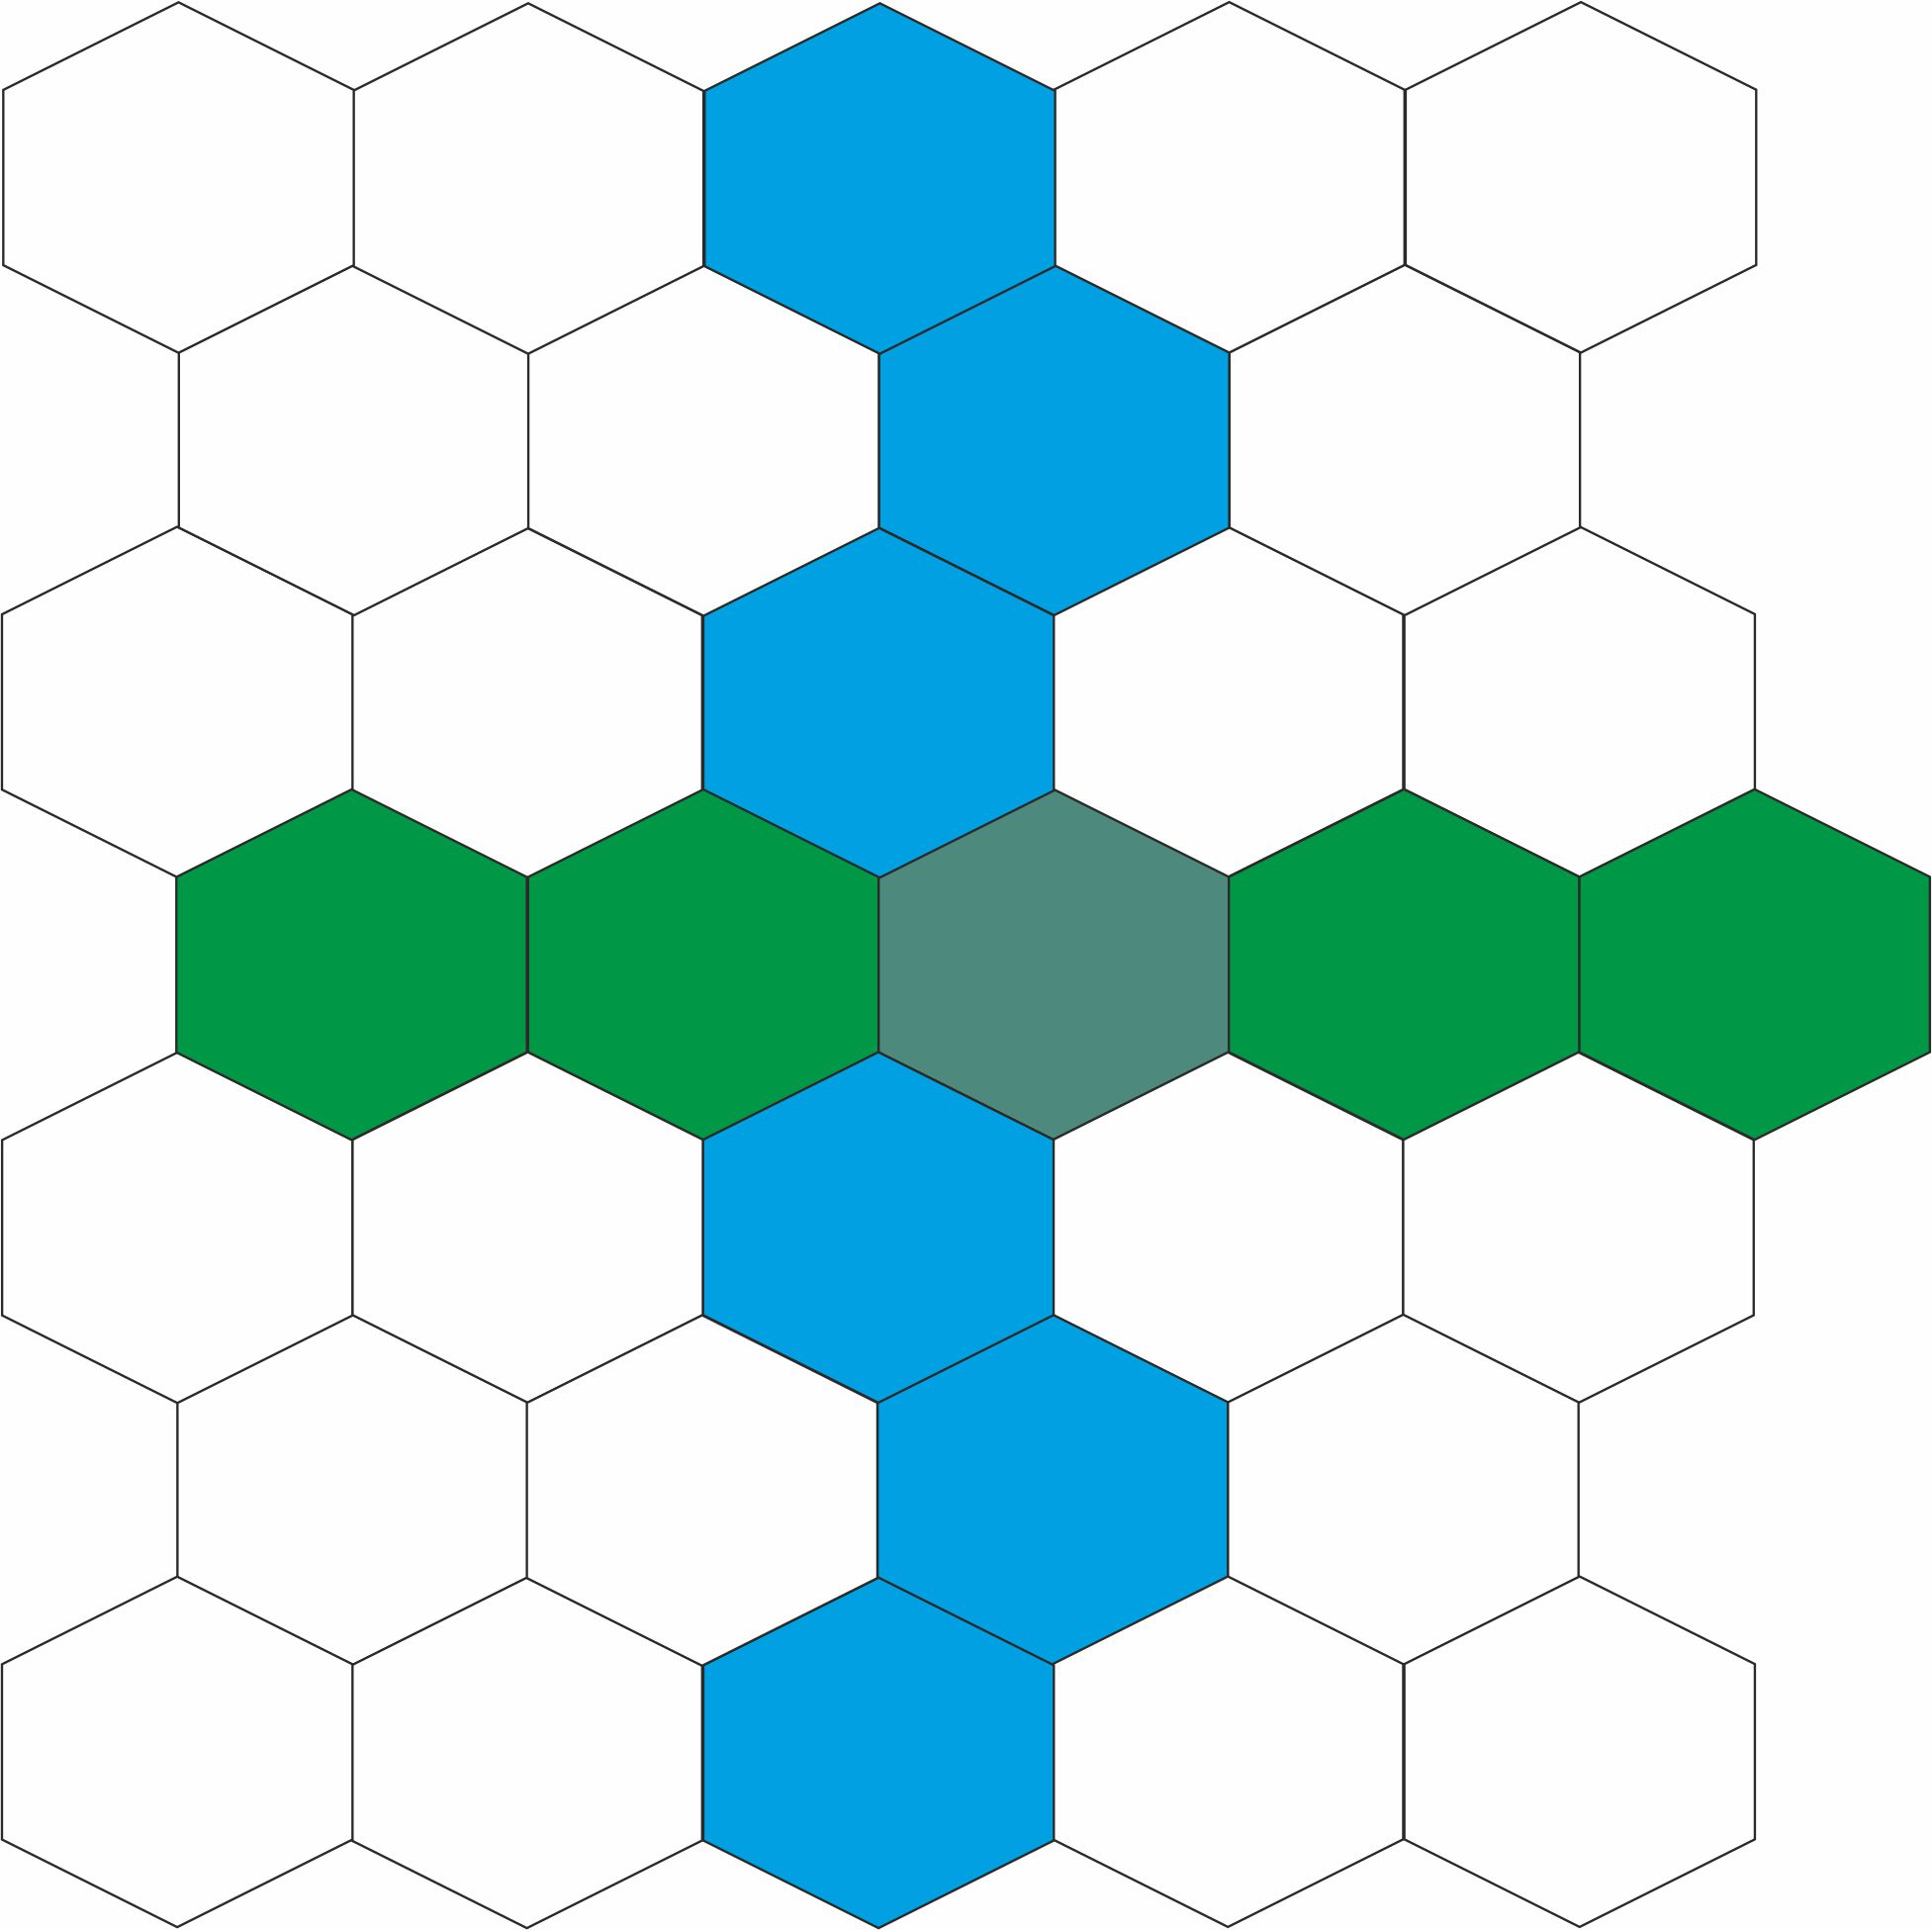
\includegraphics[scale=0.2]{kepek/OffsetCoord.jpg}
\caption{\textit{Eltolásos koordináta-rendszer}ben a tengelyek elhelyezkedése}
\label{fig:OffsetCoord}
\end{figure}

\noindent A négyzethálóval is elérhetünk a hexagonhálóhoz hasonló hatást, ha a négyzethálóban minden páros/páratlan sort/oszlopot eltolunk.

\begin{figure}[h!]
\centering
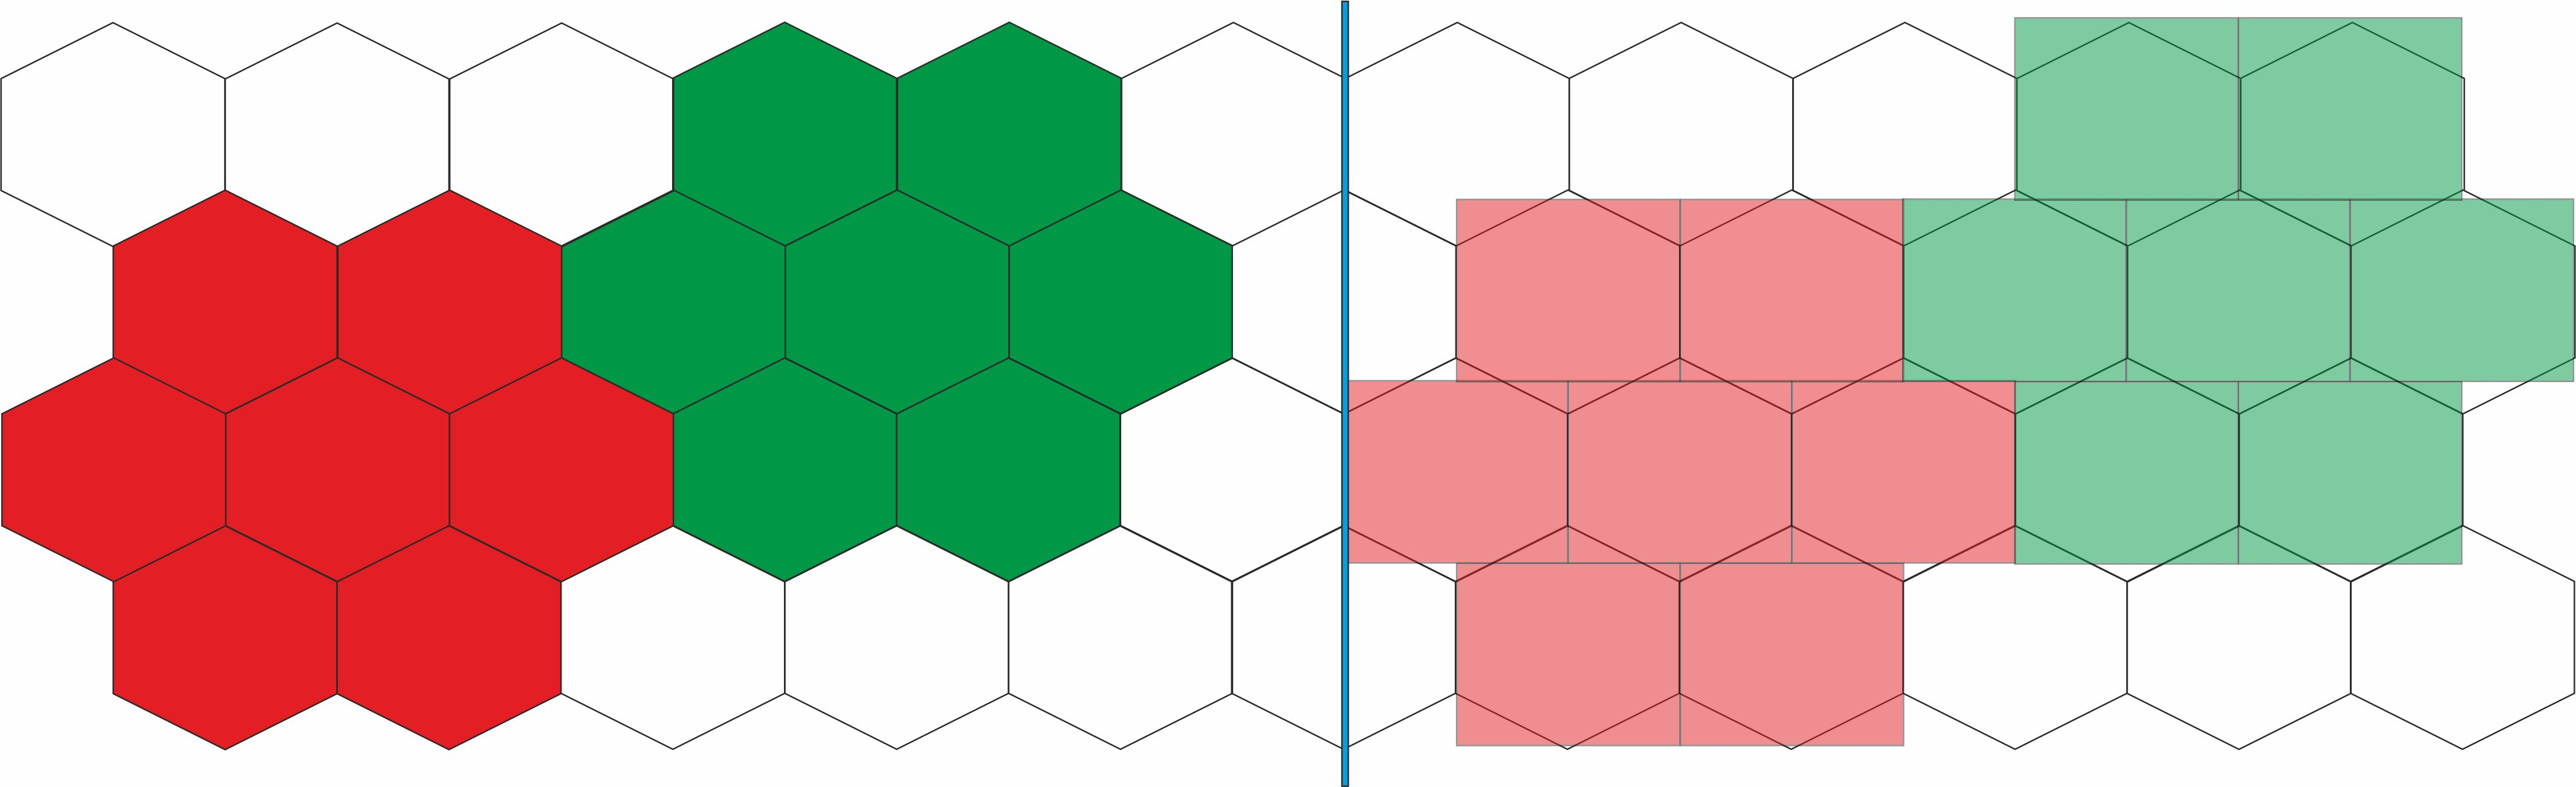
\includegraphics[scale=0.25]{kepek/Hex_Sq.jpg}
\caption{Hexagon rács az eltolt négyzetrácshoz viszonyítva}
\label{fig:Hex_Sq}
\end{figure}

\noindent Eltolható a páros és a páratlan oszlop/sor is. Mivel kétféleképpen is állhatnak a hexagonok, ezért négy fajta variáció érhető el összesen.

\begin{figure}[h!]
\centering
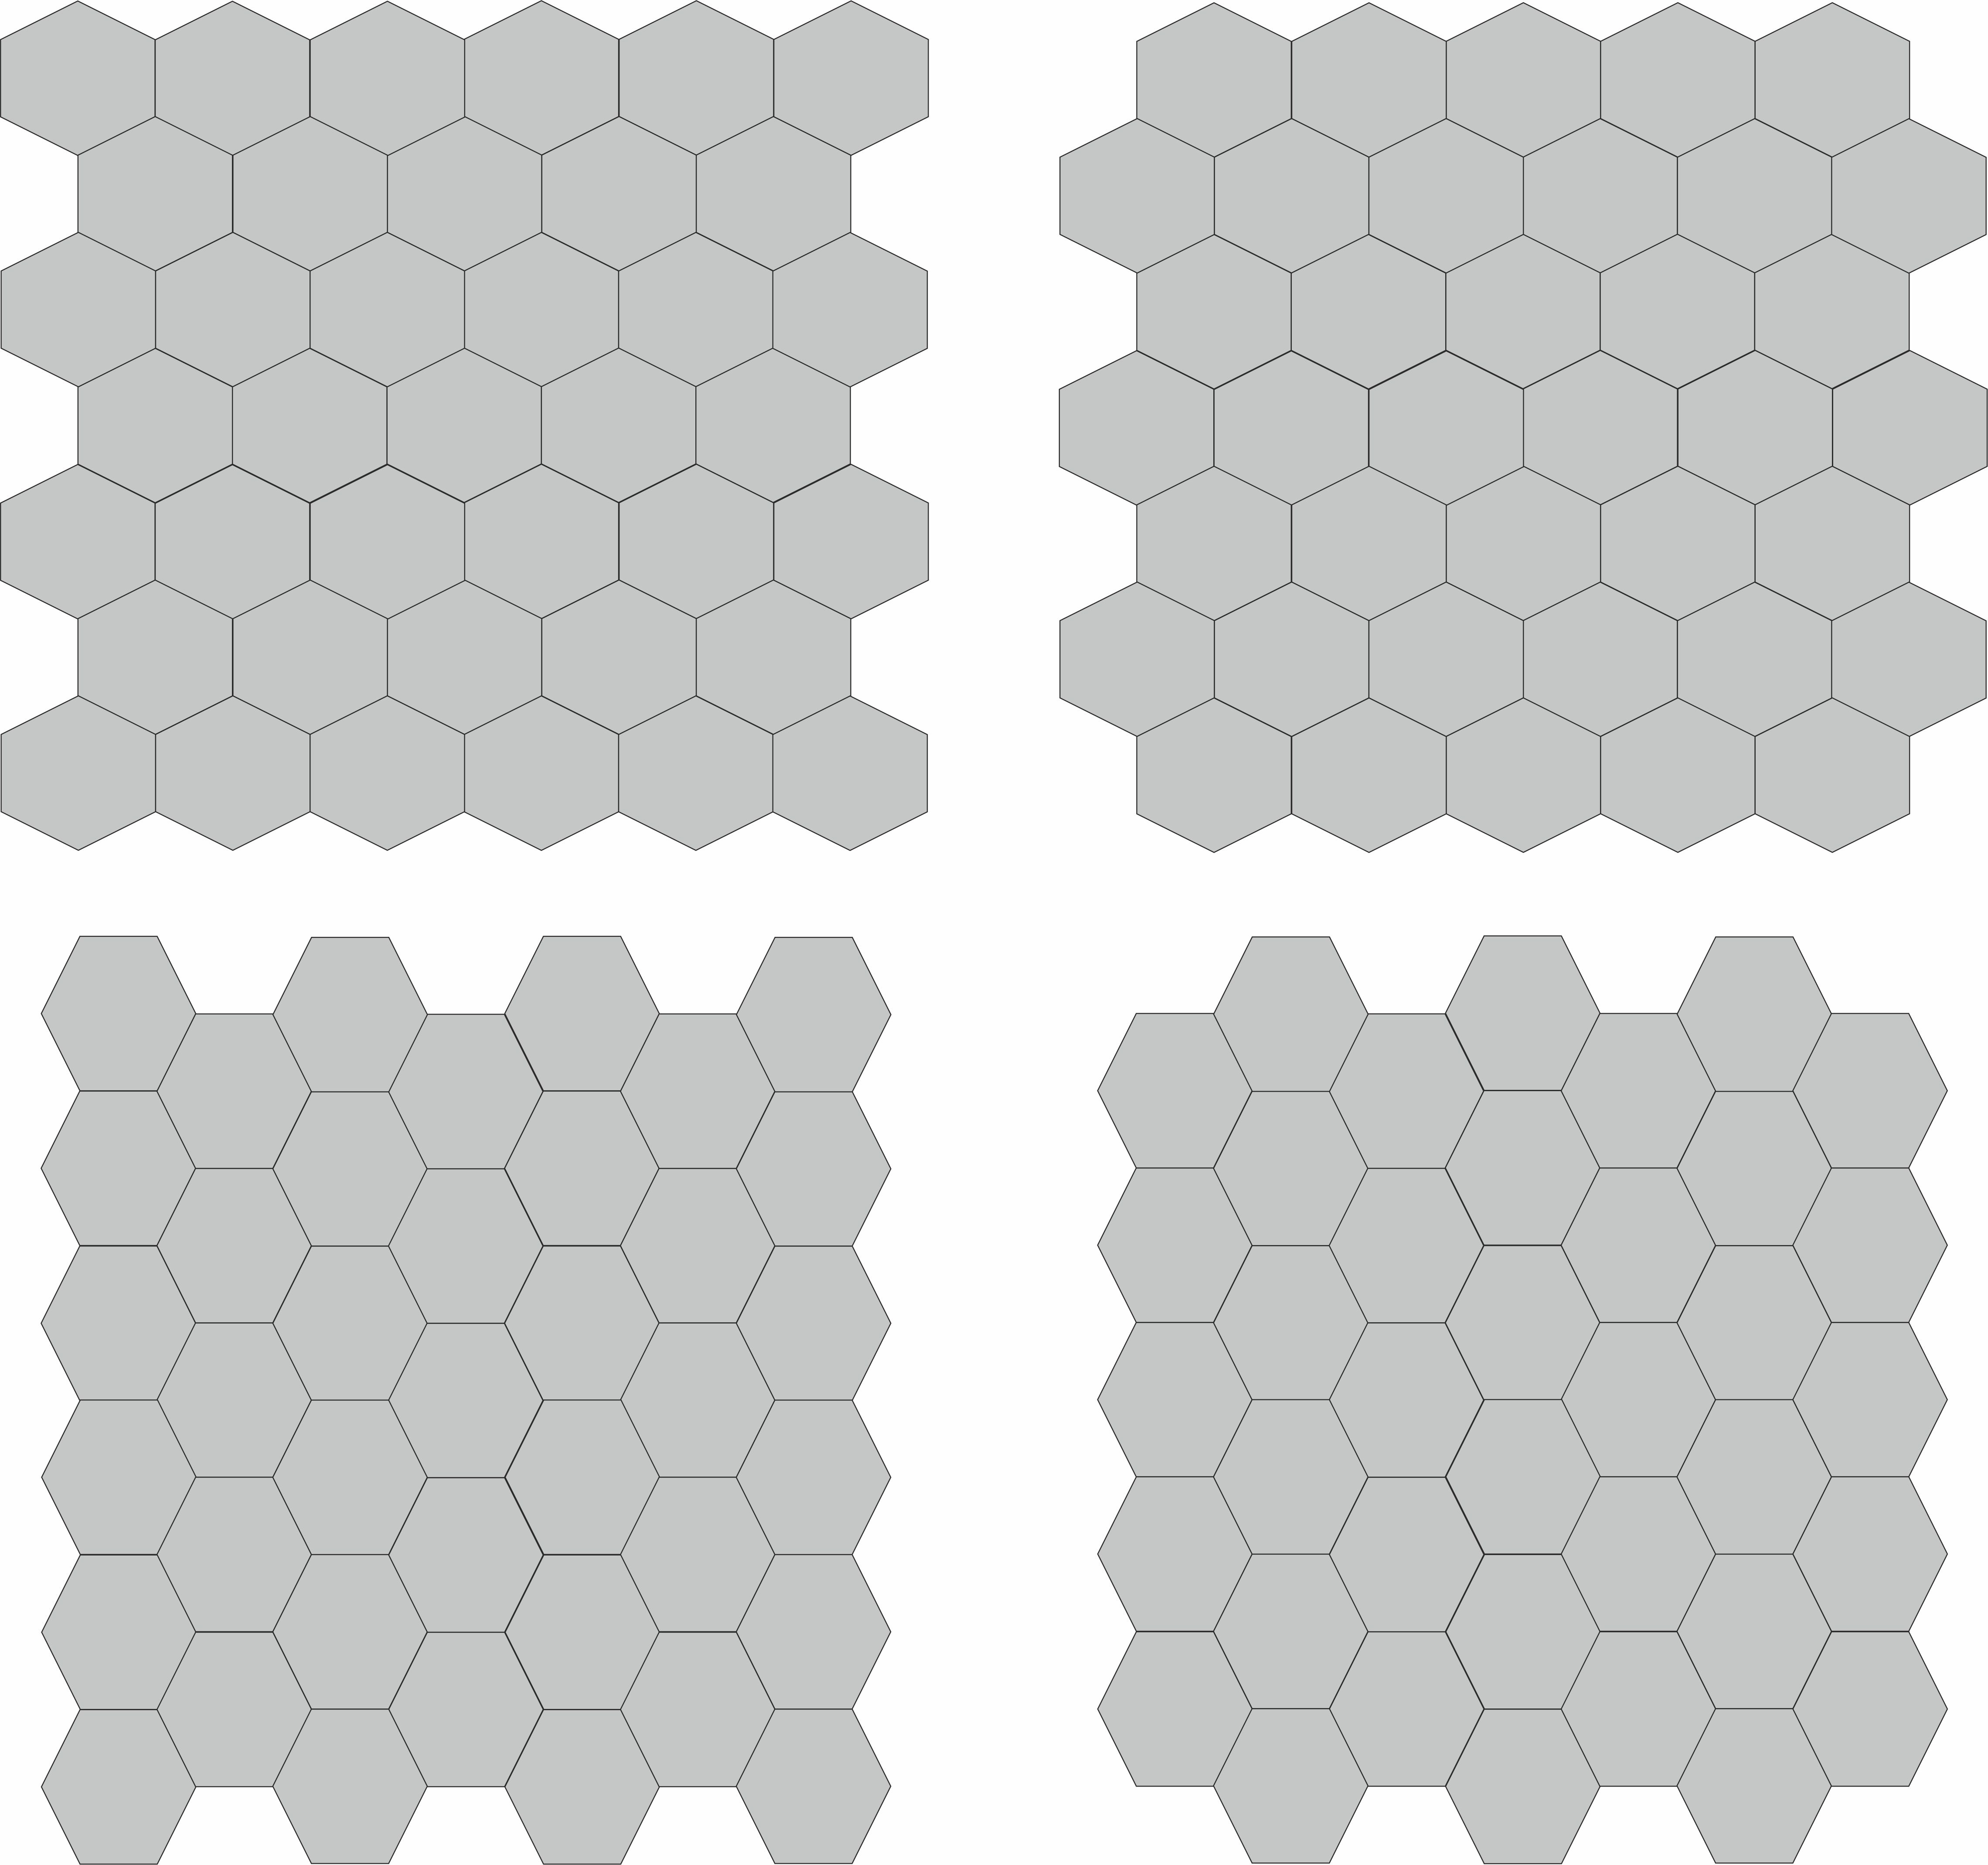
\includegraphics[scale=0.2]{kepek/OffsetFour.jpg}
\caption{A négyféle ábrázolási mód}
\label{fig:OffsetFour}
\end{figure}

\subsection{Kocka koordináta-rendszer (Cube coordinates)}

Ha egy másik fajta megközelítésből nézzük a hexagon hálókat, akkor láthatjuk, hogy három elsődleges tengelye van, nem úgy mint a korábbi koordináta-rendszereknek. 

\begin{figure}[h!]
\centering
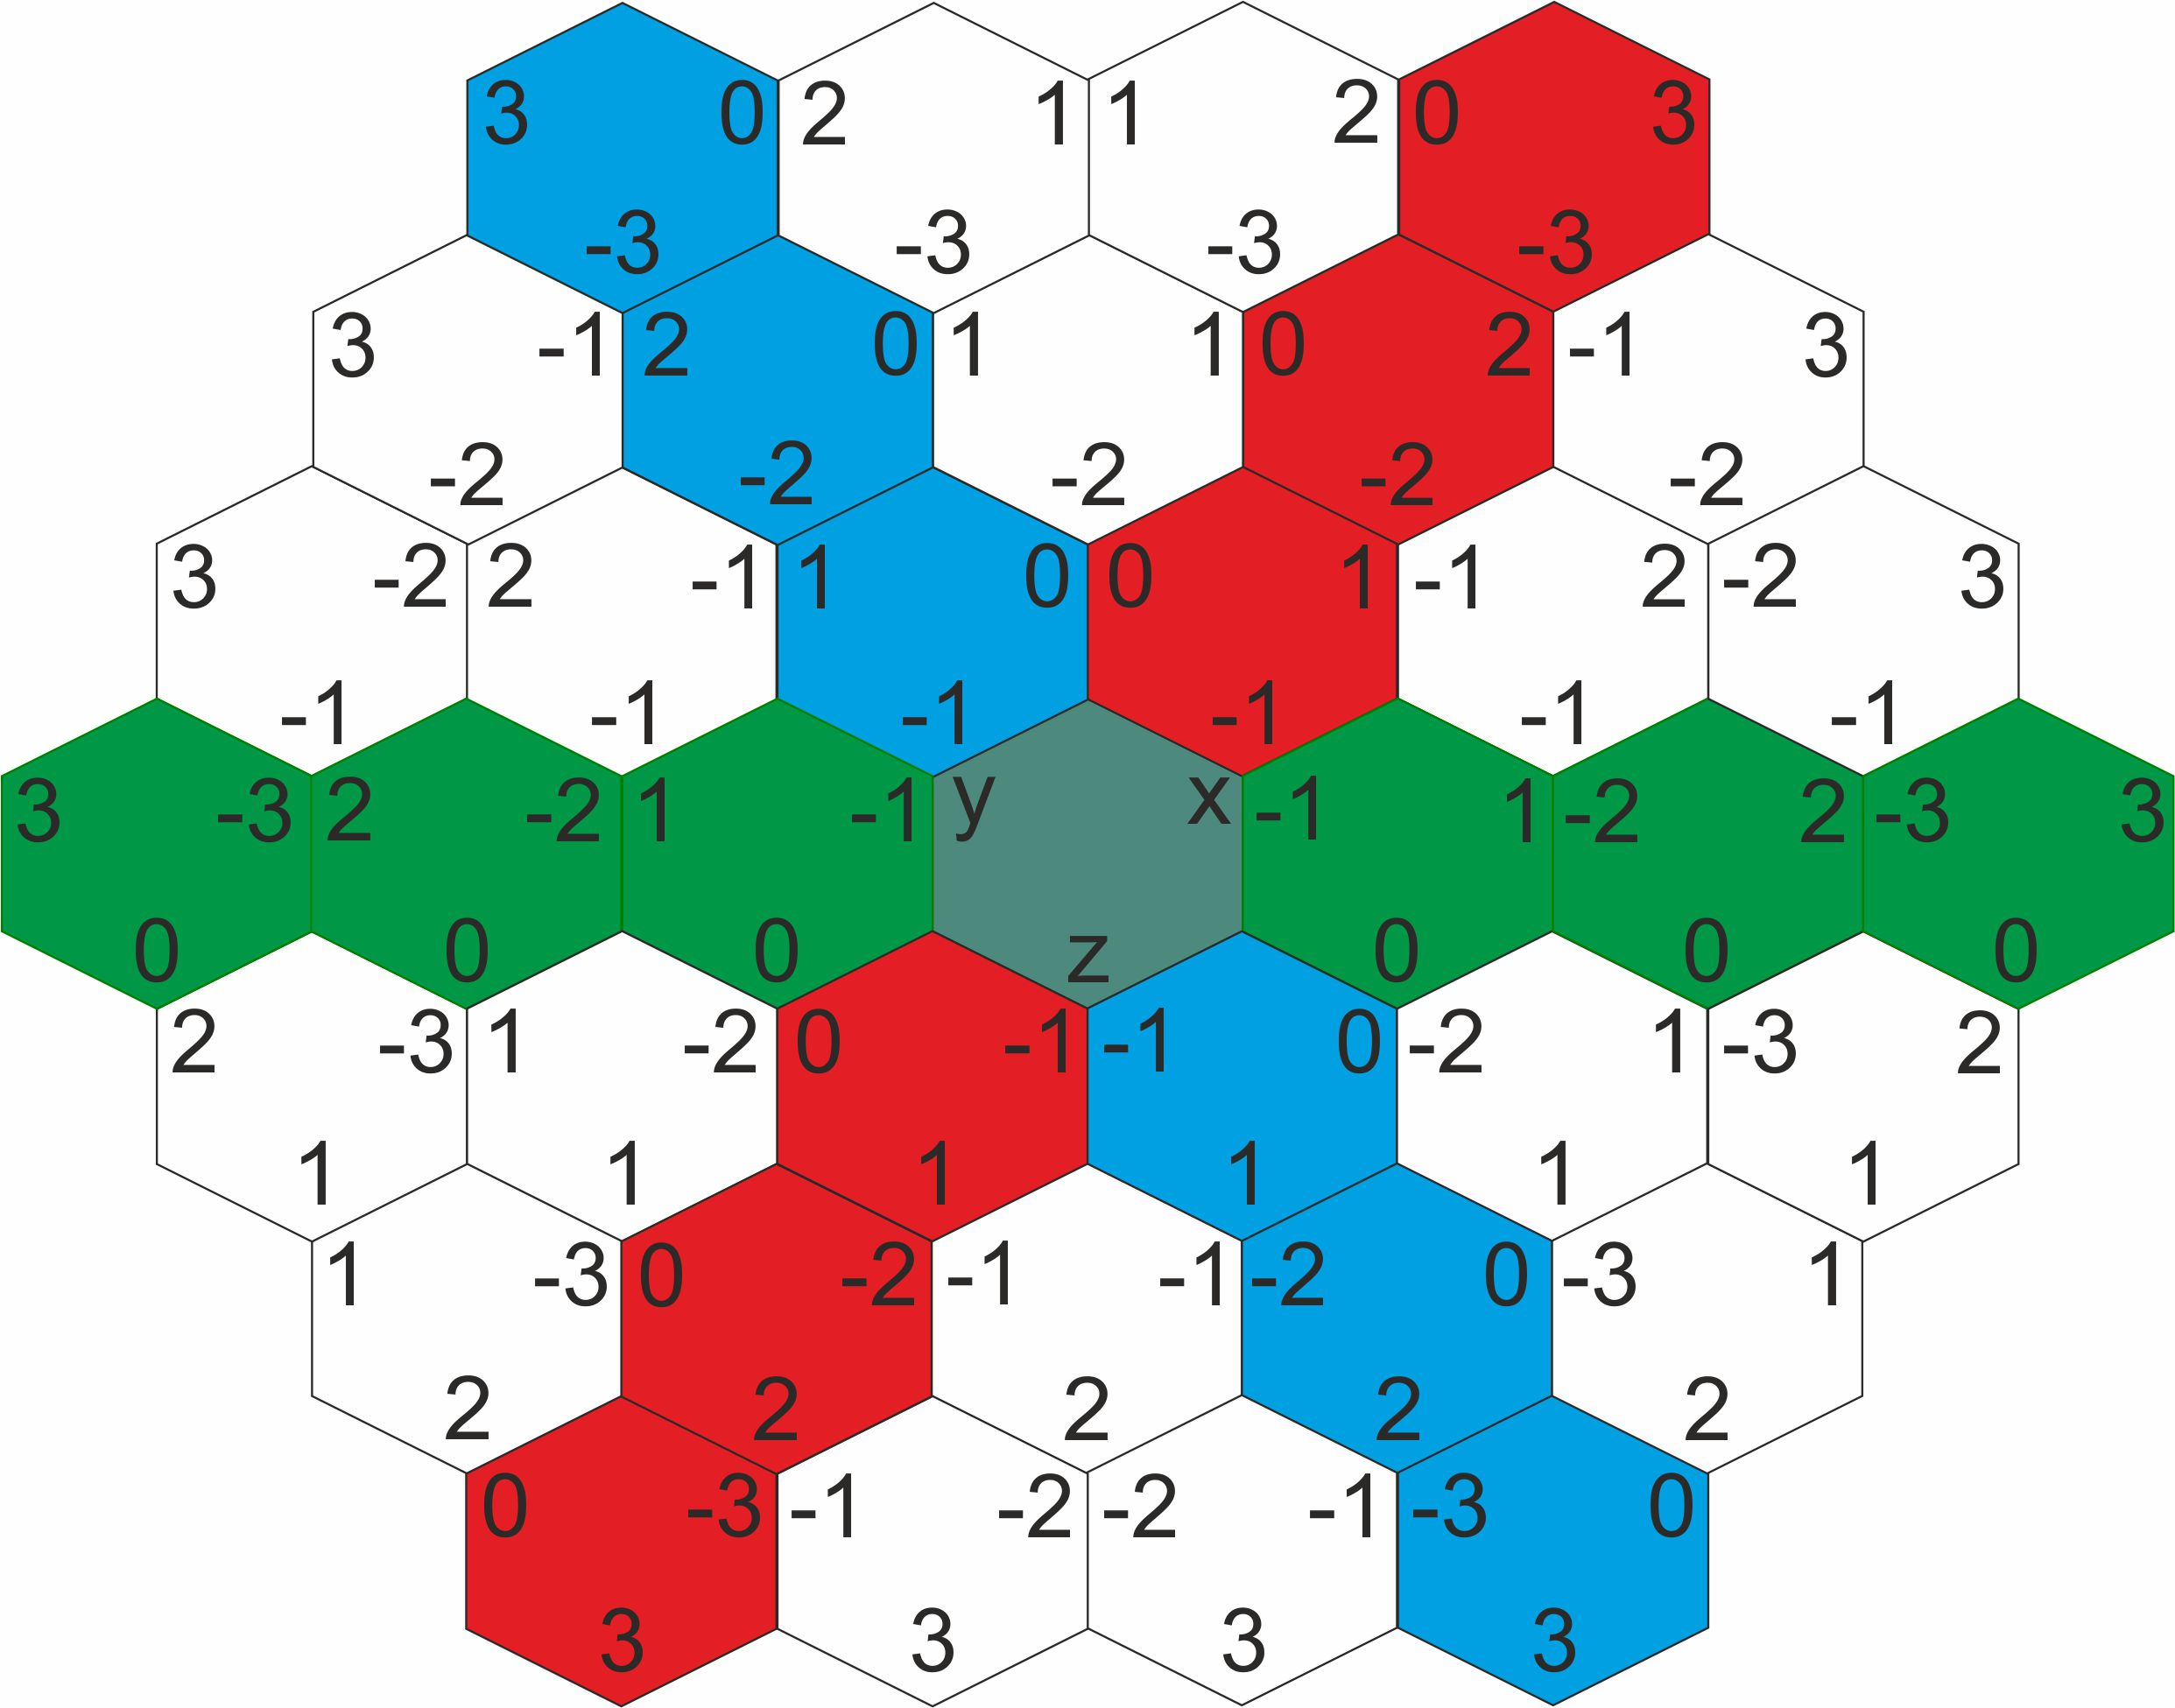
\includegraphics[scale=0.2]{kepek/CubeCoord.jpg}
\caption{A \textit{kocka koordináta rendszer}ben a tengelyek elhelyezkedése}
\label{fig:CubeCoord}
\end{figure}

\noindent Ahhoz, hogy megértsük a \textit{kocka koordináta-rendszer}t képzeljünk el egy kockarácsot és vágjunk ki belőle egy átlós síkot az $x + y + z = 0$ mentén. Ez fogja majd a hexagon rácson használt algoritmusokat egyszerűbbé tenni azáltal, hogy használhatjuk a \textit{Descartes-féle koordináta-rendszer}ben való műveleteket: hozzáadás a koordinátákhoz, kivonás a koordinátákból, szorzás vagy osztás skalárral, távolság számítás.
\newline
\newline Egy szemléletesebb példaként vizsgáljuk meg a \textit{Q*bert} nevű játékot.

\begin{figure}[h!]
\centering
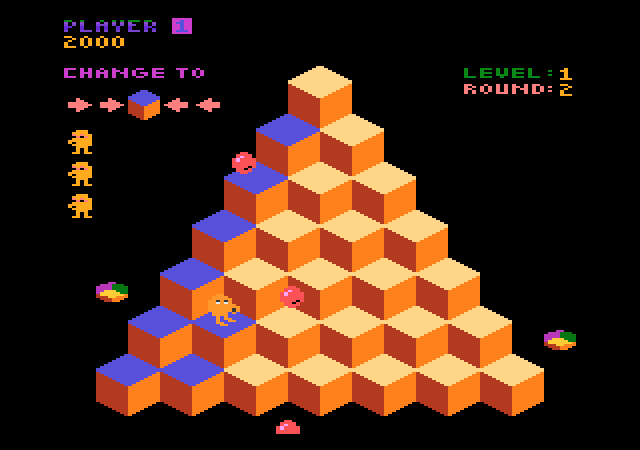
\includegraphics[scale=0.3]{kepek/Qbert.png}
\caption{A \textit{Q*bert} című játék}
\label{fig:Qbert}
\end{figure}

\noindent A játék egy $28$ kockából álló piramis szerű játékmezőn zajlik (Ilyen alakzatot kapunk, ha végrehajtjuk a fent leírtakat.). A játékos \textit{Q*bert}-et (narancssárga karakter) irányítja, aki, ha ráugrik egy kockára akkor átszínezi azt.
\newline
\newline Ha jobban megfigyeljük az ábrát, akkor láthatjuk, hogy a kockák valójában hexagonok, ha 2D-ben render-eljük, ha így nézzük, akkor \textit{Q*bert} 6 különböző irányba is léphet. Ez azt jelenti, hogy ha a párhuzamosan lévő oldalakra merőlegesen helyezünk tengelyeket, akkor hármat tudunk elhelyezni 120 fokonként.

\begin{itemize}
\item Minden hexagonnak 3 koordinátája van. 
\item Mindegyik tengely egy egyenes vonalnak felel meg a hexagon hálón.
\item Minden irány a hexagonon másik két iránynak a kombinációja a \textit{kocka koordináta-rendszer}en. Például, ha a \ref{fig:Qbert}. ábrán felfelé szeretnénk mozogni, akkor az a $+y$ és $-z$ között fekszik, ezért minden lépésnél ami felfelé történik hozzá kell adnunk 1-et az $y$-hoz és el kell vennünk 1-et a $z$-ből. 
\end{itemize}

\noindent Ez azért történik mert minden egyes mező koordinátájának az összege $0$ kell, hogy legyen ($x + y + z = 0$). Ez azt is jelenti, hogy a harmadik tengely bizonyos esetekben redundáns is lehet, például amikor meghatározzuk, hogy az egyes mezők hol jelenjenek meg a képernyőn. Ugyanakkor olyan esetekben amikor algoritmusokat (útkereső algoritmus) kell használni az előnye egyértelműen látszik (az algoritmusok könnyebb használhatósága miatt). 

\subsection{Tengely koordináta-rendszer (Axial coordinates)}

A \textit{tengely koordináta-rendszer} csak két koordinátát használ a \textit{kocka koordináta-rendszer} három koordinátája közül. Mivel a \textit{kocka koordináta-rendszer}nél volt az a megkötés, hogy $x + y + z = 0$, és ahogy a \textit{kocka koordináta-rendszer}nél már leírtam a harmadik koordináta redundáns.  A \textit{tengelyes koordináta-rendszer} használható tárolásra és megjelenítésre, mivel az $x + y + z = 0$ egyenlet alapján kiszámítható a harmadik koordináta ezért a számításokhoz is könnyen használható.

\begin{figure}[h!]
\centering
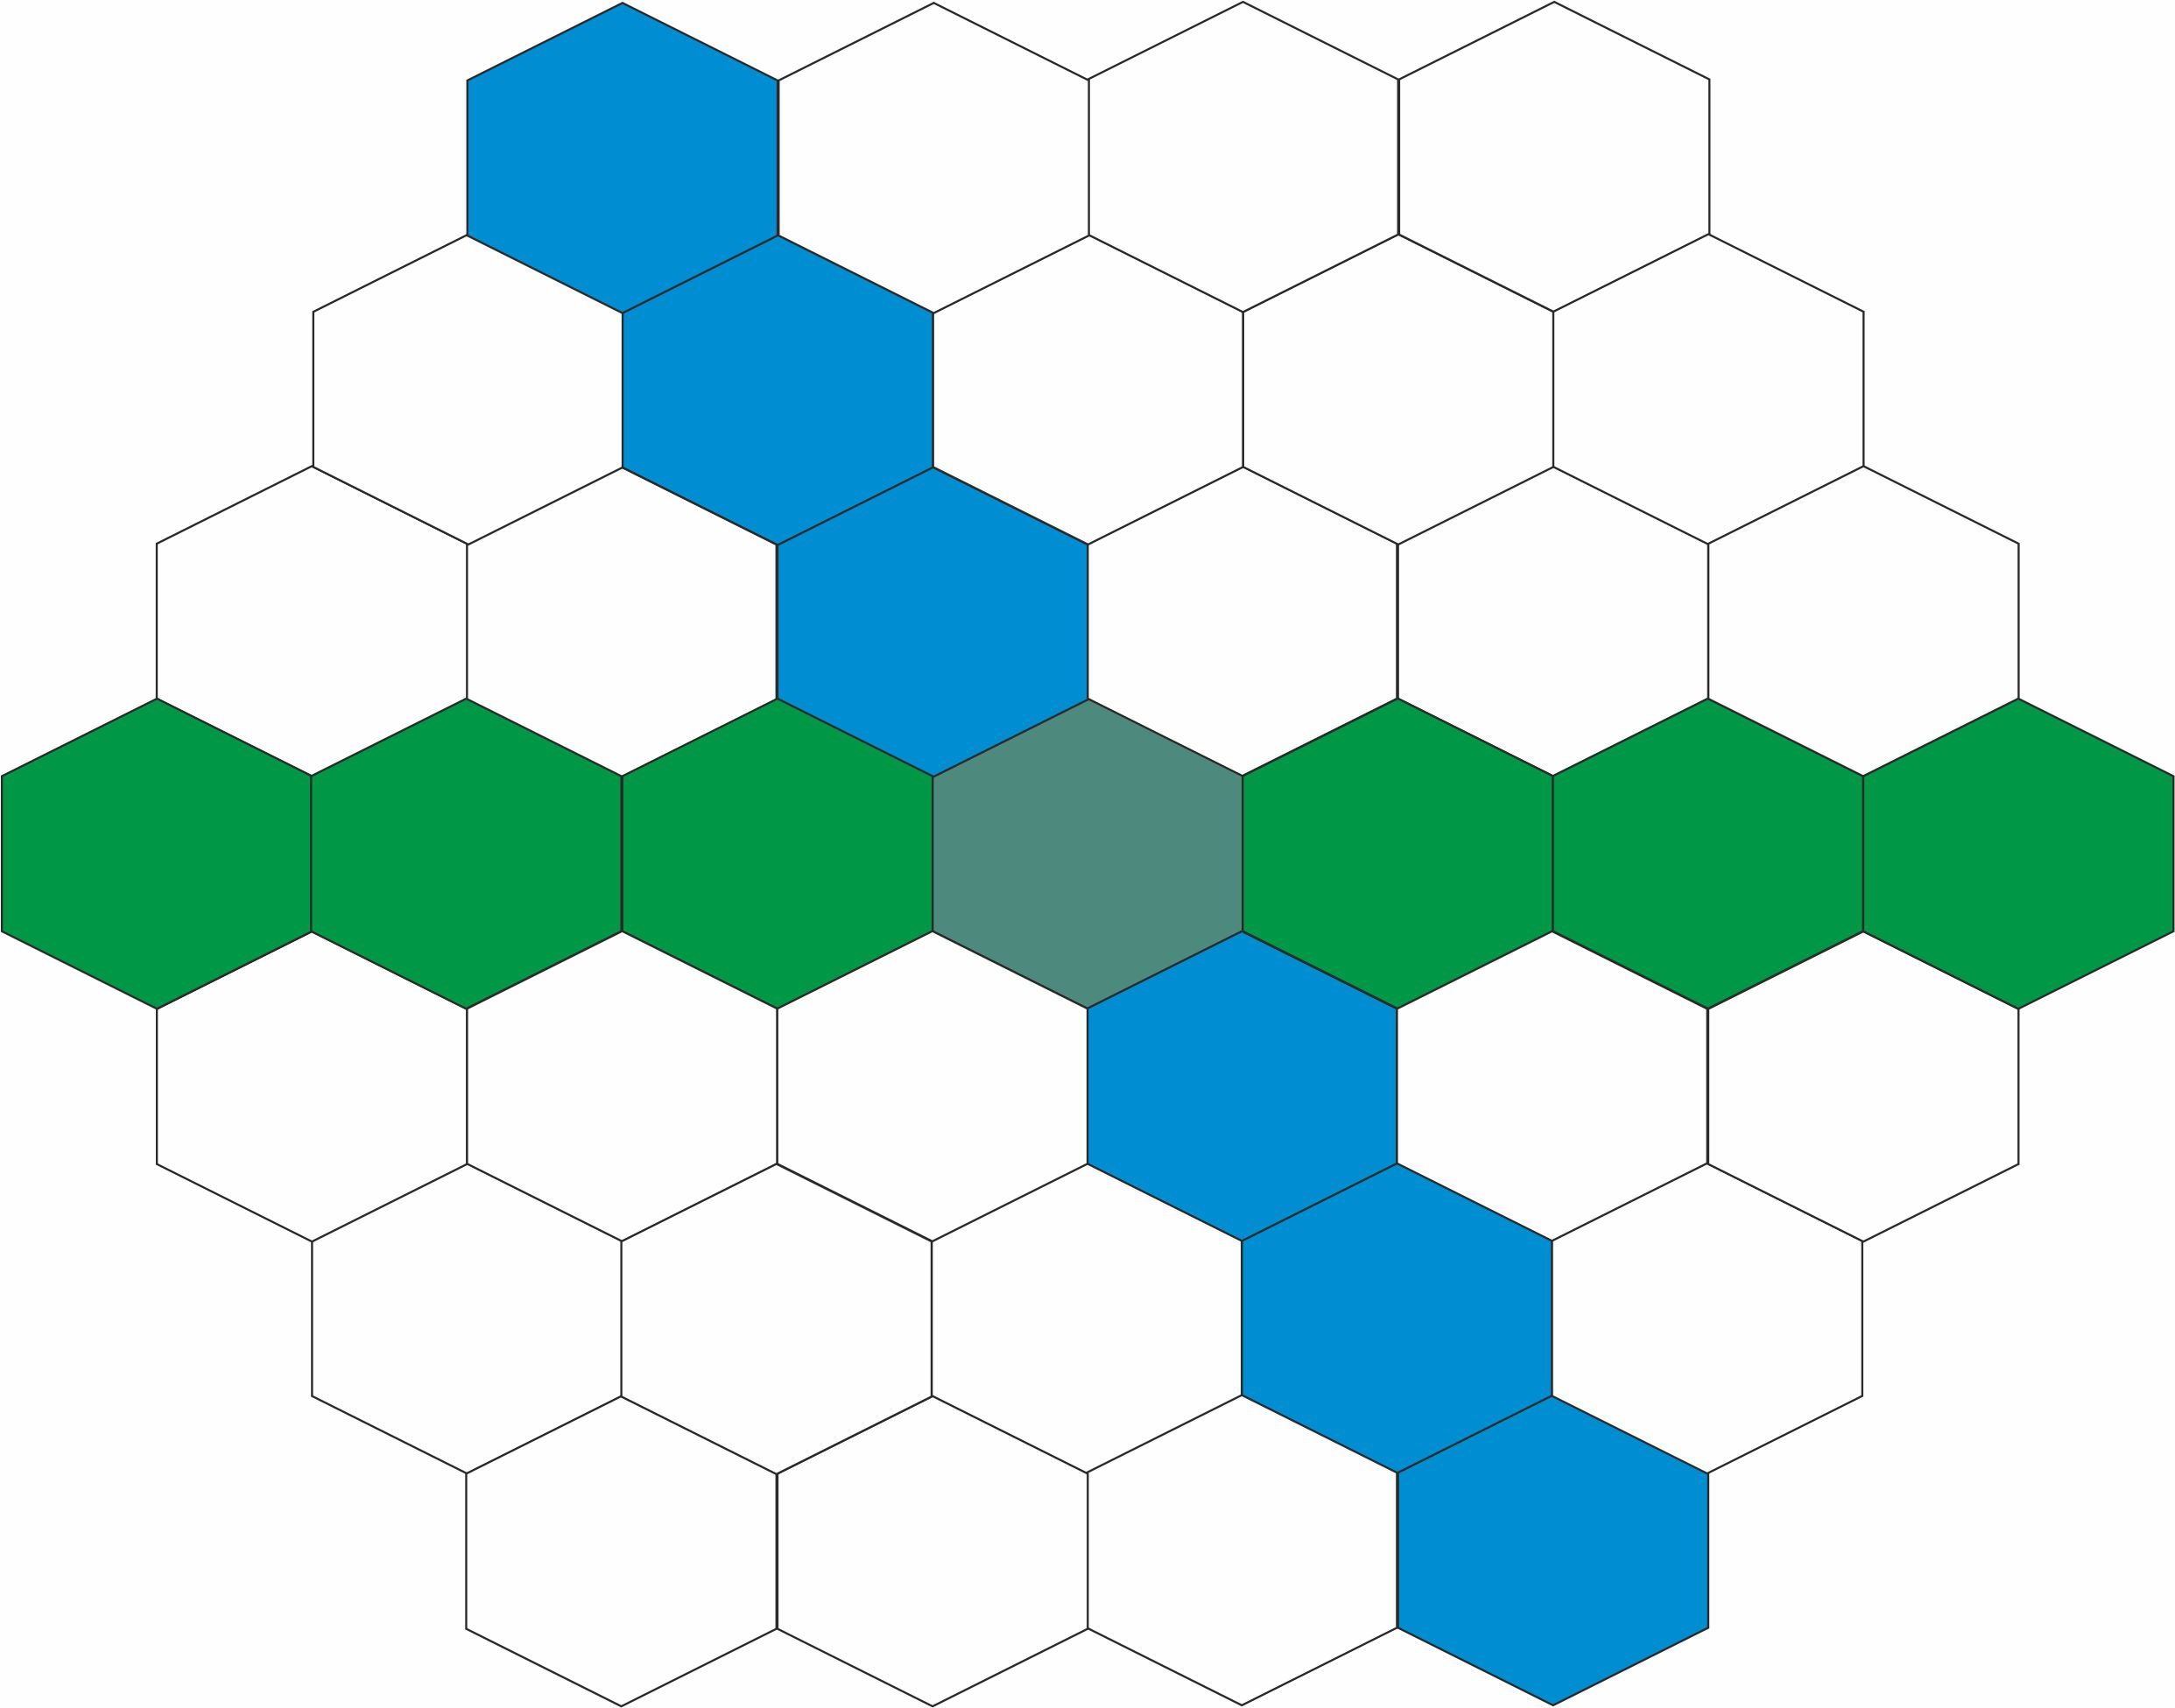
\includegraphics[scale=0.2]{kepek/AxialCoord.jpg}
\caption{A \textit{tengelyes koordináta-                                   rendszer}ben a tengelyek elhelyezkedése}
\label{fig:AxialCoord}
\end{figure}

\noindent Az előnye ennek a rendszernek az eltolásoshoz képest, hogy az algoritmusok egyszerűbbek. A hátránya ennek a rendszernek, a téglalap alakú térképek esetén való tárolás. 

\newpage 

\section{Térkép tárolási probléma}

Az egyik leggyakoribb probléma a \textit{tengelyes koordináta-rendszer}rel, hogy téglalap alakú térkép esetén elpazarolt helyek lesznek a mátrixban. Ez a fő érv az \textit{eltolásos koordináta-rendszer} mellett. Azonban az összes korábban említett koordináta-rendszer elpazarolt helyekhez vezet, amikor háromszög vagy hatszög alakú térképet használunk.
\newline

\begin{figure}[h!]
\centering
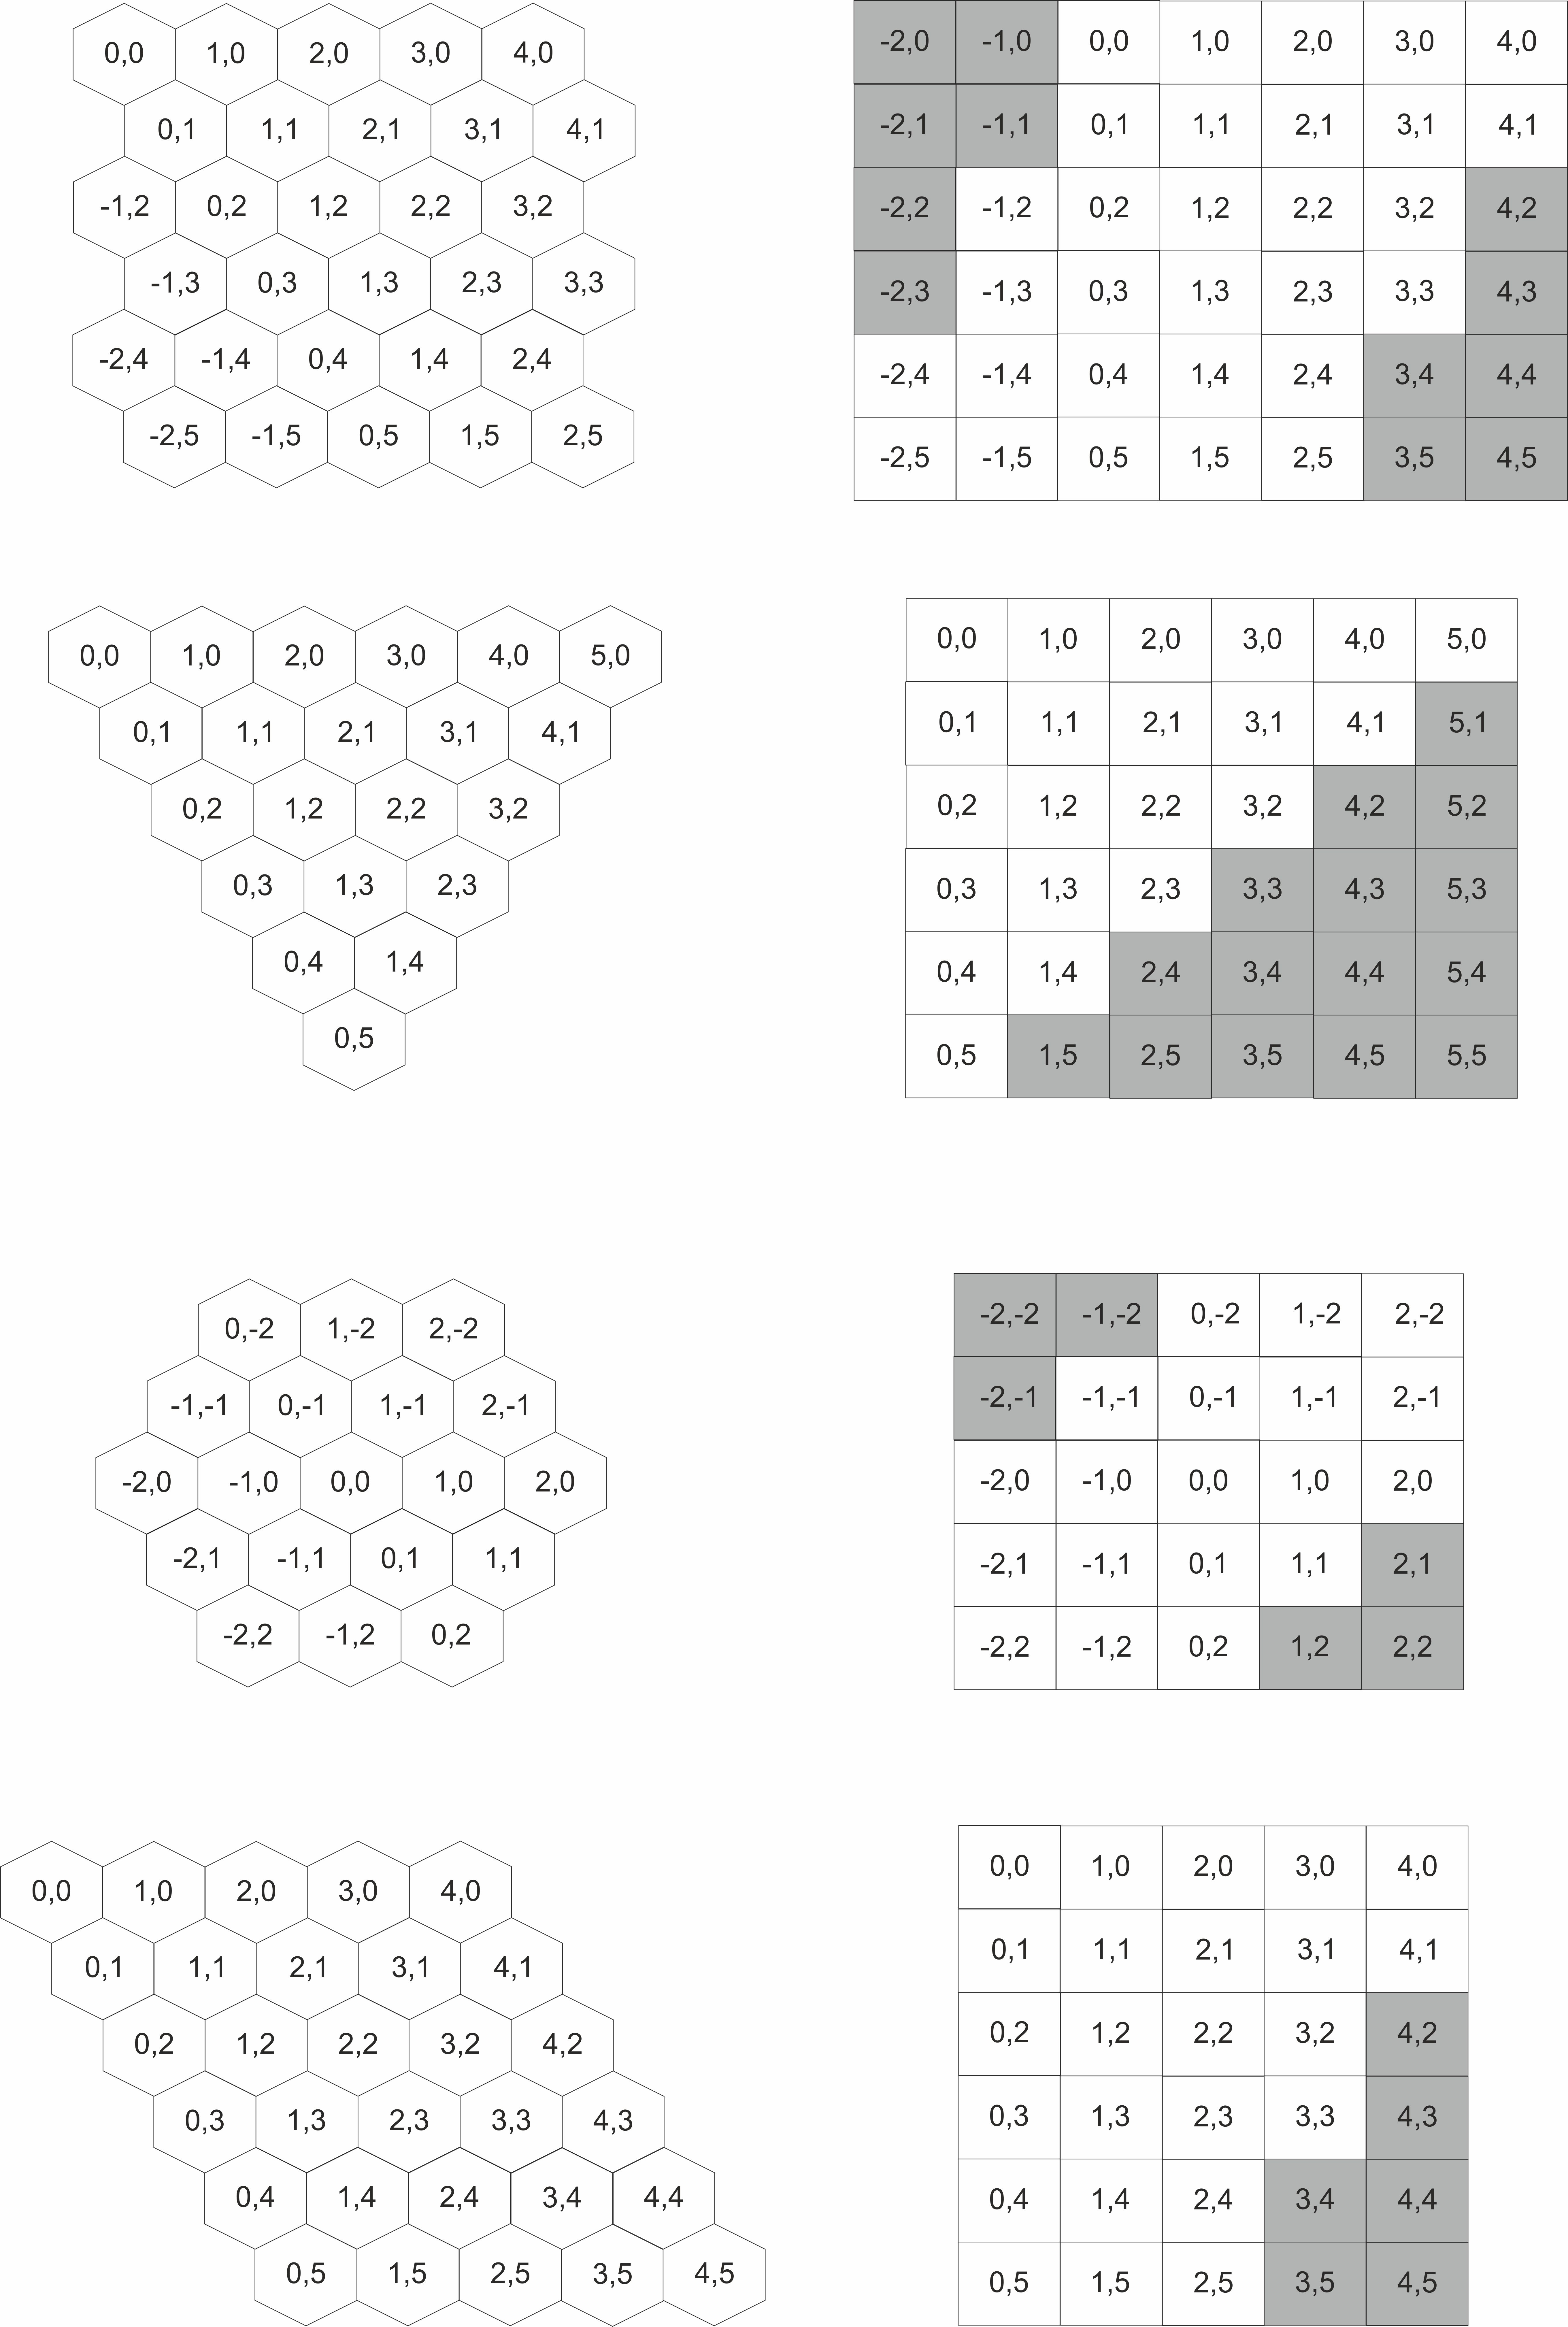
\includegraphics[scale=0.2]{kepek/StorageProblem.jpg}
\caption{Bal oldalt a különböző alakú térképek, jobb oldalt pedig a hozzájuk tárolt adat látható}
\label{fig:StorageProblem}
\end{figure}

\noindent Vegyük észre a \ref{fig:StorageProblem}. ábrán látható képeken, hogy az elpazarolt hely a sorok bal és jobb szélén jelentkezik (kivéve a rombusz esetén). Három lehetséges megoldás létezik a probléma kiküszöbölésére:
\begin{itemize}
\item Hagyjuk figyelmen kívül a problémát. Használjunk mátrixot a tárolásra és használjunk valamilyen speciális jelzőt a nem létező mezőkre. A legtöbb esetben nem éri meg ennél komplikáltabb megoldást alkalmazni.
\item Használjunk valamilyen listát a mezőkről a mátrix helyett. Ezáltal lehetőségünk lesz szabálytalan formájú térképek készítésére, beleértve azt is, hogy legyen egy lyuk a közepén. A rács osztályból getter/setter metódusok segítségével könnyen el lehet érni. (pl: $Grid(Tile(x,y))$);
\item Csúsztassuk el a sorokat úgy, hogy bal oldalt ne legyen “üres” hely. Néhány nyelvben a 2D tömb az egy tömbökből álló tömb, ilyen esetekben a tömböknek nem kell egyforma hosszúaknak lennie, így eltüntethető a felesleg a jobb oldalról is.
\newline
\newline Ahhoz, hogy ilyen különböző konvex formájú térképet tároljunk szükségünk lesz egy plusz tömbre az “első oszlopok” tárolásához. Amikor hozzá akarunk férni a hexagonhoz az q,r koordinátákon akkor az $array[r][q - elsooszlop[r]]$ kell használnunk inkább. A rács osztályból getter/setter metódusok segítségével könnyen el lehet érni.
\newline
\newline Ha a térkép fix formájú, akkor az első oszlop menet közben is számítható ahelyett, hogy tárolnánk.
\begin{itemize}
\item A téglalap alakú térképek esetén, $elsooszlop[r] == -floor(r/2)$, és ezáltal érjük el a hexagonokat úgy, hogy $grid[r][q + r/2]$, ami ekvivalens azzal mintha konvertálnánk eltolásos koordináta-rendszerbe.
\item A háromszög alakú térképek esetén, $elsooszlop[r] == 0$, és ezáltal érjük el a hexagonokat úgy, hogy $grid[r][q]$. Abban az esetben, ha a háromszög nem a képen látható módon áll, hanem csúccsal felfelé, akkor $grid[r][q + r]$.
\item A hexagon formájú $N$ sugarú térképek, ahol $N$ $=$ $max(abs(x)$, $abs(y)$, $abs(z))$, és $elsooszlop[r] == -N - min(0, r)$. Viszont hogyha $r < 0$ értékkel kezdünk, akkor el kell tolnunk a sorokat és úgy érhetjük el $grid[r + N][q + N + min(0, r)]$.
\item A rombusz formájú térkép esetén minden tökéletesen egyezik ezért egyszerűen csak a $grid[r][q]$ formát használjuk.
\end{itemize}
\end{itemize}

\section{Koordináta konverziók}

Mivel a három terület ahol a koordinátákat használjuk (tárolás, megjelenítés, számítások) nem feltétlenül ugyanabban a koordináta-rendszerben fognak megvalósulni, ezért szükséges ismernünk a különböző konverziós eljárásokat oda-vissza a különböző rendszerek között. Mivel a számításokhoz a \textit{kocka koordináta-rendszer}t fogom alkalmazni, ezért erre a rendszerre fogom alapozni az algoritmusokat.

\subsection{Tengelyes - Kocka konverziók}

A \textit{tengelyes koordináta-rendszer} nagyon közel áll a \textit{kocka koordináta-rendszer}hez. A tengelyes csak elhagyja a harmadik koordinátát, a kocka pedig kiszámolja a harmadikat a másik kettő alapján.

\begin{verbatim}
function cube_to_axial(cube):
    var q = cube.x
    var r = cube.z
    return Hex(q, r)
function axial_to_cube(hex):
    var x = hex.q
    var z = hex.r
    var y = -x-z
    return Cube(x, y, z)
\end{verbatim}

$$
axial_{q,r}(cube_{x}, cube_{y}) = 
\left \{
  \begin{tabular}{c}
  $axial_{q} = cube_{x}$ \\
  $axial_{r} = cube_{y}$
  \end{tabular}
  \right.
$$

$$
cube_{x,y,z} (axial_{q}, axial_{r}) =  \left \{
  \begin{tabular}{c}
  $cube_{x} = axial_{q}$ \\
  $cube_{z} = axial_{r}$ \\
  $cube_{y} = axial_{q} - axial_{r}$
  \end{tabular}
  \right.
$$

\subsection{Eltolásos - Kocka konverziók}

Az \textit{eltolásos koordináta-rendszer}nek négy fajta tipusa lehet, az alapján, hogy melyik sor/oszlop lett eltolva.
\newline
\newline Páratlan - sor:
\begin{verbatim}
function cube_to_oddr(cube):
      col = cube.x + (cube.z - (cube.z&1)) / 2
      row = cube.z
      return Hex(col, row)

function oddr_to_cube(hex):
      x = hex.col - (hex.row - (hex.row&1)) / 2
      z = hex.row
      y = -x-z
      return Cube(x, y, z)
\end{verbatim}

$$
oddrow_{row,col}(cube_{x},cube_{z}) = \left \{
  \begin{tabular}{c}
  $oddrow_{row} = cube_{x} + \frac{cube_{z} - (cube_{z}\; mod \; 2)}{2}$ \\
  $oddrow_{col} = cube_{z}$
  \end{tabular}
  \right.
$$

$$
cube_{x,y,z} (oddrow_{row}, oddrow_{col}) = \left \{
  \begin{tabular}{c}
  $cube_{x} = oddrow_{col} - \frac{oddrow_{row} - (oddrow_{row}\; mod \; 2)}{2}$ \\
  $cube_{y} = oddrow_{row}$ \\
  $cube_{z} = -cube_{x} - cube_{y}$
  \end{tabular}
  \right.
$$

\noindent Páros - sor:
\begin{verbatim}
function cube_to_evenr(cube):
      col = cube.x + (cube.z + (cube.z&1)) / 2
      row = cube.z
      return Hex(col, row)

function evenr_to_cube(hex):
      x = hex.col - (hex.row + (hex.row&1)) / 2
      z = hex.row
      y = -x-z
      return Cube(x, y, z)
\end{verbatim}

$$
evenrow_{row,col} (cube_{x}, cube_{z}) = \left \{
  \begin{tabular}{c}
  $evenrow_{row} = cube_{z}$ \\
  $evenrow_{col} = cube_{x} + \frac{cube_{z} + (cube_{z} \; mod \; 2)}{2}$
  \end{tabular}
  \right.
$$

$$
\scalebox{0.9}{ $cube_{x,y,z} (evenrow_{row}, evenrow_{col}) =$} \left \{
  \begin{tabular}{c}
  $cube_{x} = evenrow_{col} - \frac{evenrow_{row} + (evenrow_{row} \; mod \; 2)}{2}$ \\
  $cube_{y} = -cube_{x} - cube_{z}$ \\
  $cube_{z} = evenrow_{row}$
  \end{tabular}
  \right.
$$

\noindent Páratlan - oszlop:
\begin{verbatim}
function cube_to_oddq(cube):
      col = cube.x
      row = cube.z + (cube.x - (cube.x&1)) / 2
      return Hex(col, row)

function oddq_to_cube(hex):
      x = hex.col
      z = hex.row - (hex.col - (hex.col&1)) / 2
      y = -x-z
      return Cube(x, y, z)
\end{verbatim}

$$
oddcolumn_{row, col} (cube_{x}, cube_{z}) = \left \{
  \begin{tabular}{c}
  $oddcolumn_{row} = cube_{z} + \frac{cube_{x} - (cube_{x} \; mod \; 2)}{2}$ \\
  $oddcolumn_{col} = cube_{x}$
  \end{tabular}
  \right.
$$

$$
\scalebox{0.8}{$cube_{x,y,z} (oddcolumn_{row}, oddcolumn_{col}) =$} \left \{
  \begin{tabular}{c}
  $cube_{x} = oddcolumn_{col} $ \\
  $cube_{y} = -cube_{x} - cube_{z}$ \\
  $\scalebox{0.8}{$cube_{z} = oddcolumn_{row}$} - \frac{oddcolumn_{col} - (oddcolumn_{col} \; mod \; 2)}{2}$
  \end{tabular}
  \right.
$$

\noindent Páros - oszlop:
\begin{verbatim}
function cube_to_evenq(cube):
      col = cube.x
      row = cube.z + (cube.x + (cube.x&1)) / 2
      return Hex(col, row)

function evenq_to_cube(hex):
      x = hex.col
      z = hex.row - (hex.col + (hex.col&1)) / 2
      y = -x-z
      return Cube(x, y, z)
\end{verbatim}

$$
evencolumn_{row, col} (cube_{x}, cube_{z}) = \left \{
  \begin{tabular}{c}
  $evencolumn_{row} = cube_{z} + \frac{cube_{x} + (cube_{x} \; mod \; 2)}{2}$ \\
  $evencolumn_{col} = cube_{x}$
  \end{tabular}
  \right.
$$

$$
\scalebox{0.7}{$cube_{x,y,z} (evencolumn_{row}, evencolumn_{col}) =$} \left \{
  \begin{tabular}{c}
  $cube_{x} = evencolumn_{col} $ \\
  $cube_{y} = -cube_{x} - cube_{z}$ \\
  $\scalebox{0.7}{$cube_{z} = evencolumn_{row}$} - \frac{evencolumn_{col} + (evencolumn_{col} \; mod \; 2)}{2}$
  \end{tabular}
  \right.
$$

\noindent Érdemes \textit{bitenkénti “és”} ($a \& 1$) operátort használni \textit{modulo} ($a \% 2$) helyett, amikor megpróbáljuk meghatározni, hogy páros ($0$) vagy páratlan ($1$) sorban/oszlopban vagyunk, mivel ez működik negatív számok esetén is. Az ok nagyon egyszerű, mivel néhány nyelvben nincs lehetőség egy lépésben \textit{modulo} számítására. A maradék számítás esetén negatív számot kapnánk eredményül. 

\section{Távolság számítás}

\subsection{Kocka koordináta-rendszer}

A \textit{kocka koordináta-rendszer}ben, minden hexagon egy kockának felel meg a 3D térben. A szomszédos hexagonok 1 távolságra vannak egymástól a hexagonháló esetén, viszont 2 távolságra vannak egymástól a \textit{kocka koordináta-rendszer}ben. Ezáltal téve egyszerűvé a távolságszámítást. A \textit{négyzet koordináta-rendszer} esetén a \textit{Manhattan-távolság} képlet a következő: $abs(dx) + abs(dy)$. A \textit{kocka koordináta-rendszer}ben pedig a \textit{Manhattan-távolság} $abs(dx) + abs(dy) + abs(dz)$. Ezekből következik, hogy a hexagon rács esetén a \textit{Manhattan-távolság} képlet a kockarács esetén fennálló távolság fele.
\newline
\newline Képlettel:

$$
d_{\text{cube}}(a, b) =
\dfrac{|a_x - b_x| + |a_y - b_y| + |a_z - b_z|}{2}
$$

\noindent Egy ezzel egyenértékű megközelítés az is, ha megfigyeljük azt, hogy a három koordináta közül az egyiknek mindenképpen a a másik kettő összegének kell, hogy legyen, ekkor az az egy lesz a távolság. 
\newline
\newline Képlettel:

$$
d_{\text{cube}}(a, b) =
\max(
|a_x - b_x|, |a_y - b_y|, |a_z - b_z|
)
$$

\noindent Az, hogy melyik képletet választjuk az szituáció és egyén függő, de az eredmény ugyanaz.

\subsection{Tengelyes koordináta-rendszer}

A \textit{tengelyes koordináta-rendszer}ben a számításokhoz szükséges három koordinátából kettőt ismerünk, ezért konvertálnunk kell majd a \textit{kocka koordináta-rendszer}re.
\newline
\newline Képlettel:

$$
d_{hex}(a, b) = \frac{|a.x - b.x| + |a.x + a.y - b.x - b.y| + |a.z - b.z|}{2}
$$

\subsection{Eltolásos koordináta-rendszer}

Az \textit{eltolásos koordináta-rendszer} esetén azt a megoldást fogjuk használni, hogy átalakítjuk a koordinátákat a \textit{kocka koordináta-rendszer}re.
\newline
\newline Képlettel:

$$
d_{of\!fset} (a, b) = d_{cube}(of\!fset\_to\_Cube(a), of\!fset\_to\_Cube(b)) 
$$

